
\Act*{3}
\Scene{1}[Before \textsc{Prospero's} Cell.]

\begin{figure}[t!]
\centering
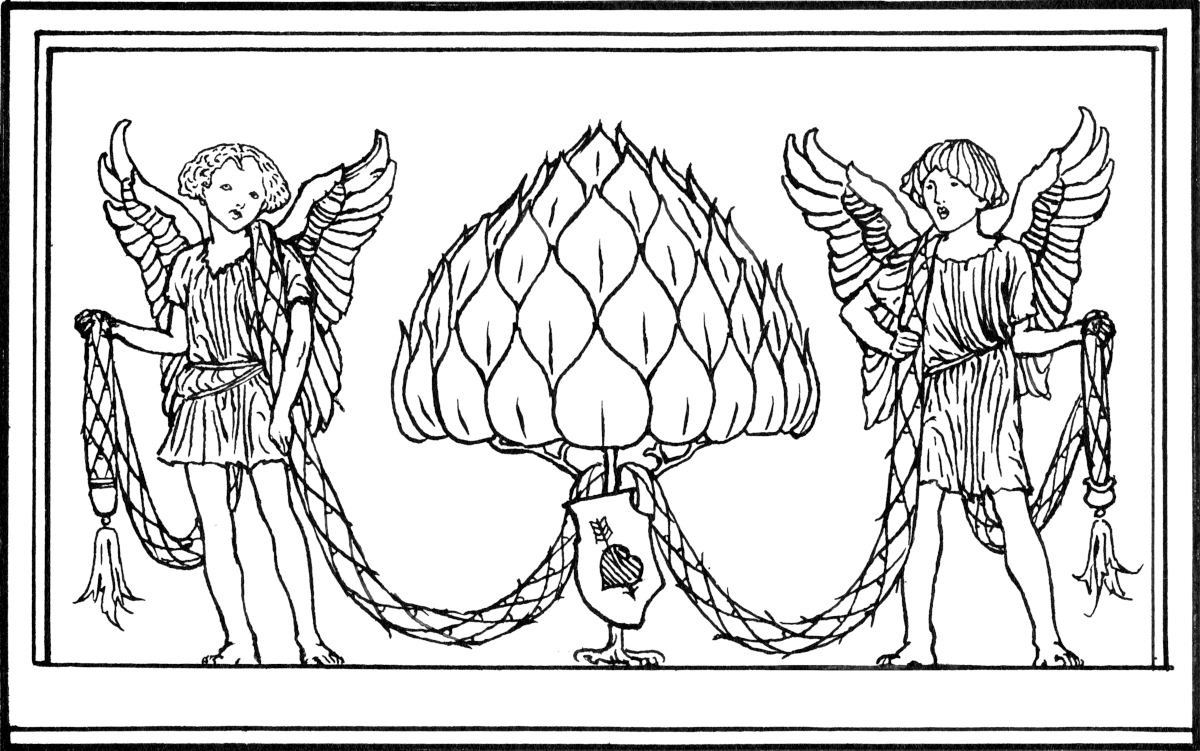
\includegraphics[width=\headerwidth]{3iheadpiece}
\end{figure}

\enter{\textsc{Ferdinand}, bearing a log}

\begin{letter} %dropcap
	\begin{tikzpicture}[remember picture, overlay]
		\node (dropcap) at ($(current page.west)+(2.5cm,-3cm)$) {
\includegraphics[width=0.125\linewidth]{3idropcapT}};
	\end{tikzpicture}
\end{letter}

\begin{a4} %dropcap
	\begin{tikzpicture}[remember picture, overlay]
		\node (dropcap) at ($(current page.west)+(2.5cm,-2.3cm)$) {
\includegraphics[width=0.12\linewidth]{3idropcapT}};
	\end{tikzpicture}
\end{a4}
	
\begin{verse_speech}[Ferdinand] 
\hspace{1em}here be some sports are painful, and their labour\\
\hspace{1em}Delight in them sets off: some kinds of baseness\\
Are nobly undergone and most poor matters\\
Point to rich ends. This my mean task\\
Would be as heavy to me as odious, but\\
The mistress which I serve quickens what's dead\\
And makes my labours pleasures: O, she is\\
Ten times more gentle than her father's crabbed,\\
And he's composed of harshness. I must remove\\
Some thousands of these logs and pile them up,\\
Upon a sore injunction: my sweet mistress\\
Weeps when she sees me work, and says, such baseness\\
Had never like executor. I forget:\\
But these sweet thoughts do even refresh my labours,\\
Most busy lest, when I do it.
\end{verse_speech}

\begin{figure}[tb]
\centering
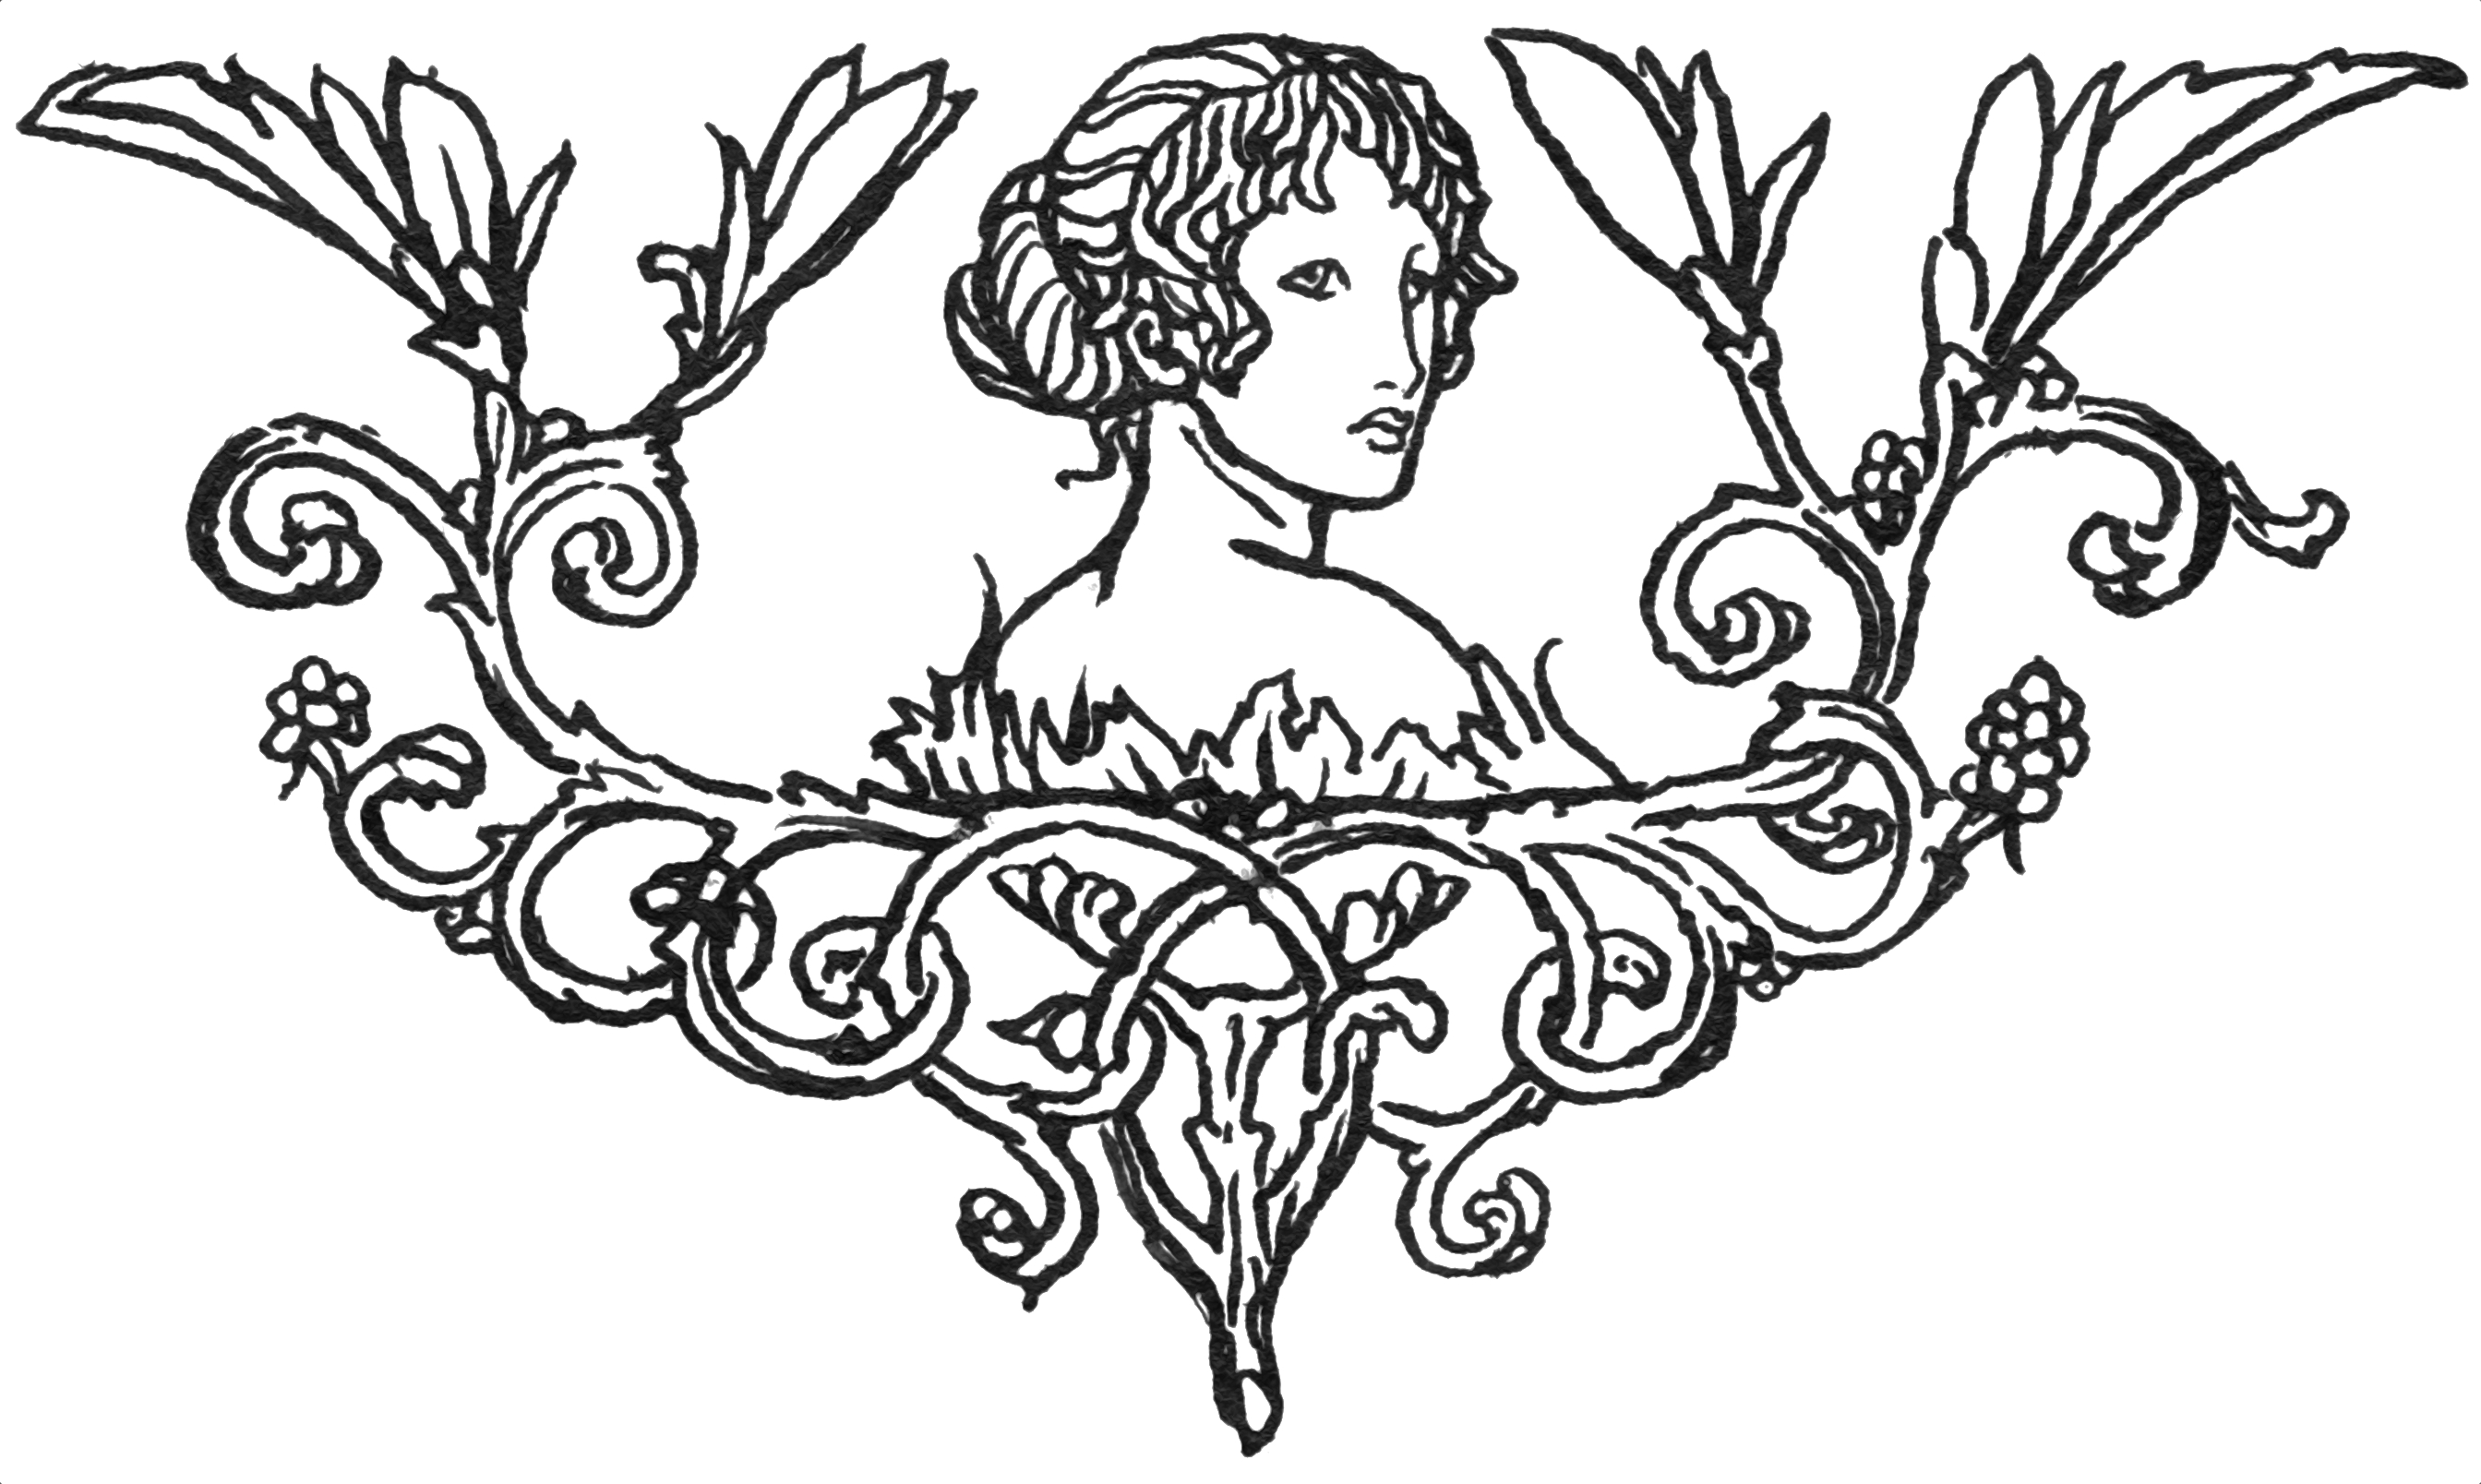
\includegraphics[width=\smallwidth]{3itail1}
\end{figure}



\enter{\textsc{Miranda}; and \textsc{Prospero} at a distance, unseen}

\begin{verse_speech}[Miranda] 
\hspace{\widthof{Most busy lest, when I do it.}}Alas, now, pray you,\\
Work not so hard: I would the lightning had\\
Burnt up those logs that you are enjoin'd to pile!\\
Pray, set it down and rest you: when this burns,\\
'Twill weep for having wearied you. My father\\
Is hard at study; pray now, rest yourself;\\
He's safe for these three hours.
\end{verse_speech}

\begin{verse_speech}[Ferdinand] 
\hspace{\widthof{He's safe for these three hours.}}O most dear mistress,\\
The sun will set before I shall discharge\\
What I must strive to do.
\end{verse_speech}

\begin{verse_speech}[Miranda] 
\hspace{\widthof{What I must strive to do.}}If you'll sit down,\\
I'll bear your logs the while: pray, give me that;\\
I'll carry it to the pile.
\end{verse_speech}

\begin{verse_speech}[Ferdinand] 
\hspace{\widthof{I'll carry it to the pile.}}No, precious creature;\\
I had rather crack my sinews, break my back,\\
Than you should such dishonour undergo,\\
While I sit lazy by.
\end{verse_speech}

\begin{verse_speech}[Miranda] 
\hspace{\widthof{While I sit lazy by.}}It would become me\\
As well as it does you: and I should do it\\
With much more ease; for my good will is to it,\\
And yours it is against.
\end{verse_speech}

\begin{verse_speech}[Prospero] 
\hspace{\widthof{And yours it is against.}}Poor worm, thou art infected!\\
This visitation shows it.
\end{verse_speech}

\verseline[Miranda]{\hspace{\widthof{This visitation shows it.}}You look wearily.}

\begin{verse_speech}[Ferdinand] 
No, noble mistress; 'tis fresh morning with me\\
When you are by at night. I do beseech you—\\
Chiefly that I might set it in my prayers—\\
What is your name?
\end{verse_speech}

\begin{verse_speech}[Miranda] 
\hspace{\widthof{What is your name?}}Miranda.—O my father,\\
I have broke your hest to say so!
\end{verse_speech}

\begin{verse_speech}[Ferdinand] 
\hspace{\widthof{I have broke your hest to say so!}}Admired Miranda!\\
Indeed the top of admiration! worth\\
What's dearest to the world! Full many a lady\\
I have eyed with best regard and many a time\\
The harmony of their tongues hath into bondage\\
Brought my too diligent ear: for several virtues\\
Have I liked several women; never any\\
With so fun soul, but some defect in her\\
Did quarrel with the noblest grace she owed\\
And put it to the foil: but you, O you,\\
So perfect and so peerless, are created\\
Of every creature's best!
\end{verse_speech}

\begin{figure}[tb]
\centering
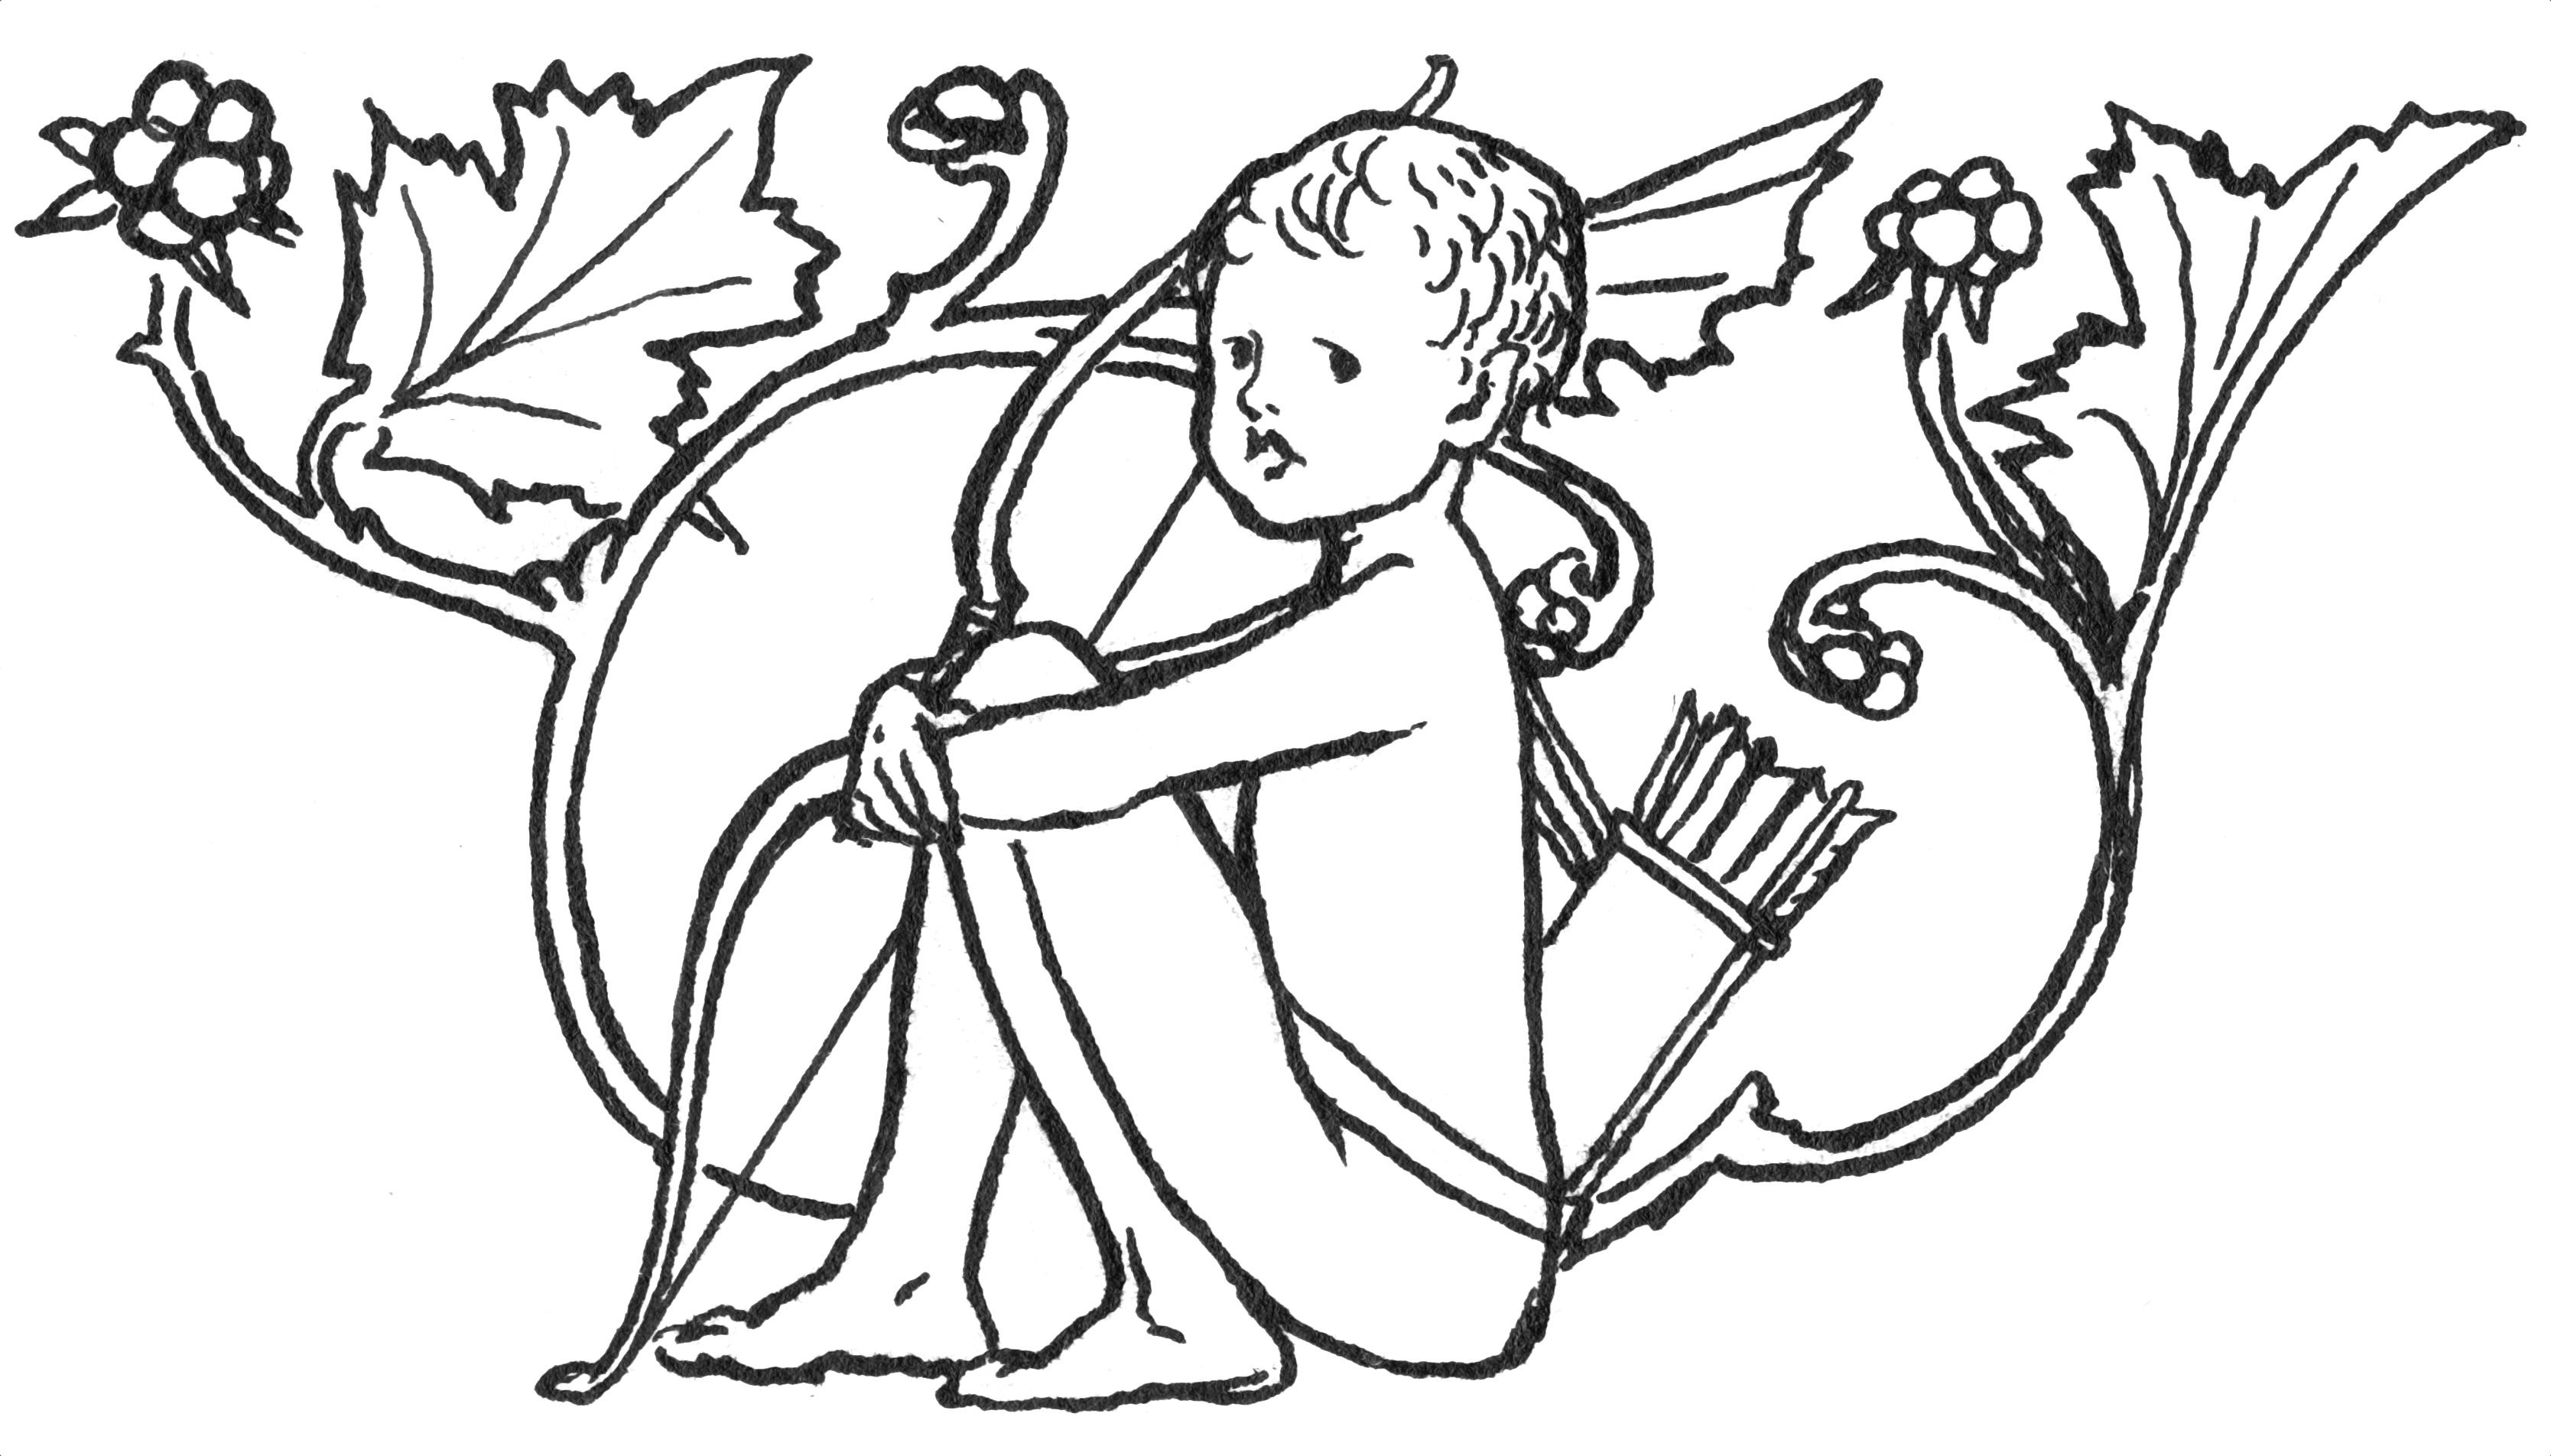
\includegraphics[width=\smallwidth]{cupid}
\end{figure}

\begin{verse_speech}[Miranda] 
\hspace{\widthof{Of every creature's best!}}I do not know\\
One of my sex; no woman's face remember,\\
Save, from my glass, mine own; nor have I seen\\
More that I may call men than you, good friend,\\
And my dear father: how features are abroad,\\
I am skilless of; but, by my modesty,\\
The jewel in my dower, I would not wish\\
Any companion in the world but you,\\
Nor can imagination form a shape,\\
Besides yourself, to like of. But I prattle\\
Something too wildly and my father's precepts\\
I therein do forget.
\end{verse_speech}

\begin{verse_speech}[Ferdinand] 
I am in my condition\\
A prince, Miranda; I do think, a king;\\
I would, not so!—and would no more endure\\
This wooden slavery than to suffer\\
The flesh-fly blow my mouth. Hear my soul speak:\\
The very instant that I saw you, did\\
My heart fly to your service; there resides,\\
To make me slave to it; and for your sake\\
Am I this patient log-man.
\end{verse_speech}

\verseline[Miranda]{Do you love me?}

\begin{verse_speech}[Ferdinand] 
O heaven, O earth, bear witness to this sound\\
And crown what I profess with kind event\\
If I speak true! if hollowly, invert\\
What best is boded me to mischief! I\\
Beyond all limit of what else i' the world\\
Do love, prize, honour you.
\end{verse_speech}

\begin{verse_speech}[Miranda] 
I am a fool\\
To weep at what I am glad of.
\end{verse_speech}

\begin{verse_speech}[Prospero] 
Fair encounter\\
Of two most rare affections! Heavens rain grace\\
On that which breeds between 'em!
\end{verse_speech}

\verseline[Ferdinand]{Wherefore weep you?}

\begin{verse_speech}[Miranda] 
At mine unworthiness that dare not offer\\
What I desire to give, and much less take\\
What I shall die to want. But this is trifling;\\
And all the more it seeks to hide itself,\\
The bigger bulk it shows. Hence, bashful cunning!\\
And prompt me, plain and holy innocence!\\
I am your wife, it you will marry me;\\
If not, I'll die your maid: to be your fellow\\
You may deny me; but I'll be your servant,\\
Whether you will or no.
\end{verse_speech}

\begin{verse_speech}[Ferdinand] 
My mistress, dearest;\\
And I thus humble ever.
\end{verse_speech}

\verseline[Miranda]{My husband, then?}

\begin{verse_speech}[Ferdinand] 
Ay, with a heart as willing\\
As bondage e'er of freedom: here's my hand.
\end{verse_speech}

\begin{verse_speech}[Miranda] 
And mine, with my heart in't; and now farewell\\
Till half an hour hence.
\end{verse_speech}

\verseline[Ferdinand]{A thousand thousand!}

\exit{\textsc{Ferdinand} and \textsc{Miranda} severally}

\begin{verse_speech}[Prospero] 
So glad of this as they I cannot be,\\
Who are surprised withal; but my rejoicing\\
At nothing can be more. I'll to my book,\\
For yet ere supper-time must I perform\\
Much business appertaining.
\end{verse_speech}
\exit{}

\begin{figure}[b]
\centering

\includegraphics[width=\headerwidth]{3itail2}
\end{figure}

	% \begin{tikzpicture}[remember picture, overlay]
		% \node (dropcap) at ($(current page.south)+(0cm,2.5cm)$) {
\includegraphics[width=.6\textwidth]{3itail2}};
	% \end{tikzpicture}
	